% Define document class
\documentclass[twocolumn]{aastex631}

% Filler text
\usepackage{blindtext}

\newcommand{\tess}{\textit{TESS}}
\newcommand{\sname}{V1298~Tau}
\newcommand{\allplanets}{V1298~Tau~bcd}
\newcommand{\planetb}{V1298~Tau~b}
\newcommand{\planetc}{V1298~Tau~c}
\newcommand{\planetd}{V1298~Tau~d}
\newcommand{\planete}{V1298~Tau~e}
\newcommand{\rearth}{$R_\oplus$}
\newcommand{\exoplanet}{\texttt{exoplanet}}




% Begin!
\begin{document}

% Title
\title{Updated Ephemerides of the young multi-planet system V1298 Tau from TESS}

% Author list
\author[0000-0002-9464-8101]{Adina~D.~Feinstein}
\altaffiliation{NSF Graduate Research Fellow}
\affiliation{Department of Astronomy and Astrophysics, University of Chicago, Chicago, IL 60637, USA}

\author[0000-0001-6534-6246]{Trevor J.\ David}
\affiliation{Center for Computational Astrophysics, Flatiron Institute, New York, NY 10010, USA}
\affiliation{Department of Astrophysics, American Museum of Natural History, New York, NY 10024, USA}

\author[0000-0001-7516-8308]{Benjamin~T.~Montet}
\affiliation{School of Physics, University of New South Wales, Sydney, NSW 2052, Australia}
\affiliation{UNSW Data Science Hub, University of New South Wales, Sydney, NSW 2052, Australia}

\author[0000-0002-4881-3620]{John~H.~Livingston}
\affiliation{Department of Astronomy, University of Tokyo, 7-3-1 Hongo, Bunkyo-ku, Tokyo 113-0033, Japan}

\author{Charles Beichman}
\affiliation{Caltech/IPAC, 1200 E. California Blvd. Pasadena, CA 91125, USA}


\author[0000-0002-3199-2888]{Sarah Blunt}
\altaffiliation{NSF Graduate Research Fellow}
\affiliation{Department of Astronomy, California Institute of Technology, Pasadena, CA, USA}


\author{DFM?}

\correspondingauthor{Adina~D.~Feinstein;\\ \twitter{afeinstein20}; \github{afeinstein20};} \email{afeinstein@uchicago.edu} 

% Abstract with filler text
\begin{abstract}
    \blindtext
\end{abstract}

% Main body with filler text
\section{Introduction}


%%%%%%%%%%%%%%%%%%%%%%%%%%%%%%%%%%%%%%%%%%%%%%%%%%%%%%%
\begin{figure*}[!ht]
\begin{center}
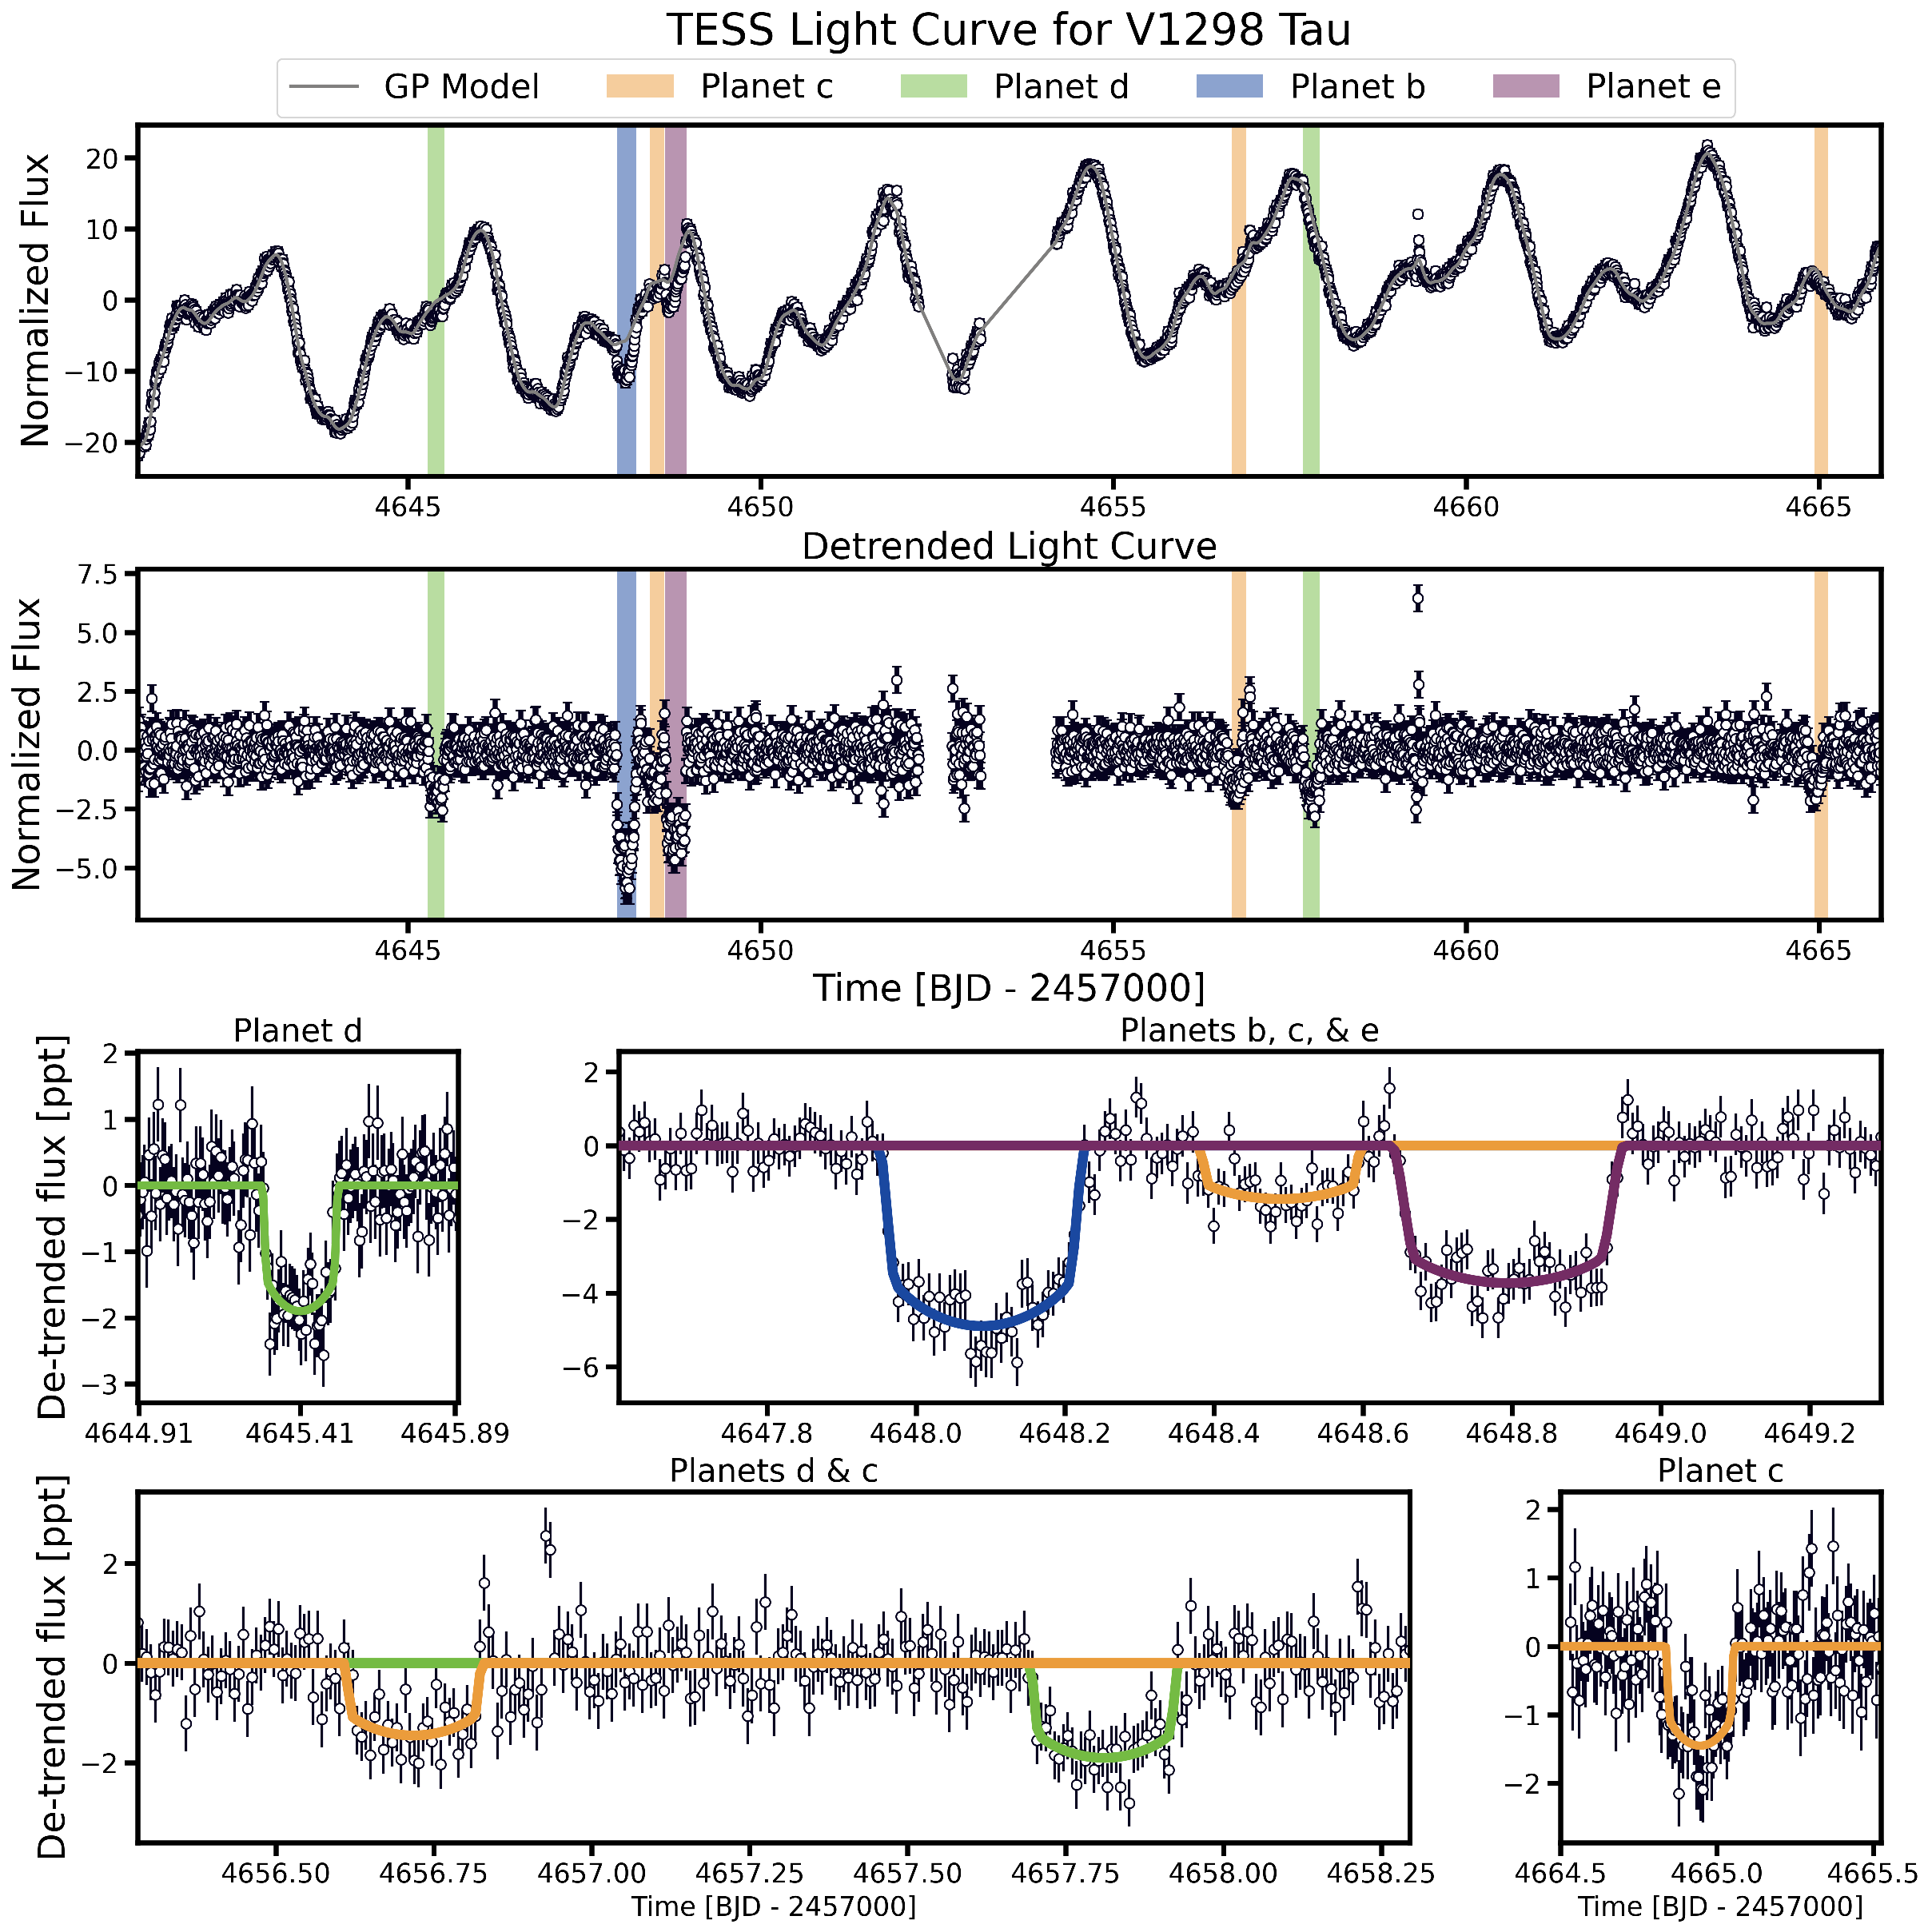
\includegraphics[width=\textwidth,trim={0.25cm 0 0 0}]{figures/lightcurve.pdf}
\caption{\sname extracted light curve from the \texttt{tica}-processed full-frame images, with transits of \allplanets highlighted by color. Top row: extracted light curve with over plotted with our best-fit GP model for stellar variability (black). Middle row: the \tess\ light curve with the stellar variability removed by our model. Bottom rows: zoomed-in regions around the visible transits during the first orbit (third row) and second orbit (last row) from \tess\ Sector 43. \label{fig:transits}}
\end{center}
\end{figure*}
%%%%%%%%%%%%%%%%%%%%%%%%%%%%%%%%%%%%%%%%%%%%%%%%%%%%%%%

\end{document}
